\documentclass{article}
\usepackage[utf8]{inputenc}   % Allows accents directly like á, é, ñ
\usepackage[T1]{fontenc}      % Proper font encoding
\usepackage{amsmath}
\usepackage{amsthm}
\usepackage{amssymb}
\usepackage{graphicx}
\usepackage{hyperref}
\renewcommand\qedsymbol{$\blacksquare$}
\graphicspath{ {./Images/} }


\title{Situación Problema: Fundamentos del Álgebra Lineal}
\author{Ricardo Salgado Benítez - A01282489 \\ Tecnológico de Monterrey \\ Docente: Jesús Jorge Armenta Segura}
\date{12 de septiembre de 2025}

\begin{document}
\maketitle
\newpage
\section{Resumen}

En este reporte, se presenta un método para llevar a cabo códigos de Hamming mediante herramientas de álgebra lineal, a diferencia de los métodos tradicionales que recurren a operadores lógicos. Las herramientas en cuestión son el campo de Galois \{0, 1\}, las matrices y la multiplicación de estas últimas. La primera sección de este reporte, explica el problema que se busca resolver mediante los códigos de Hamming. La segunda sección aborda las herramientas del álgebra lineal referidas anteriormente. La siguiente sección es el núcleo del reporte y explica el método que fue usado para implementar los códigos de Hamming. Posteriormente, se abordan las conclusiones de este reporte. Finalmente, se incluyen anexos que contienen una implementación del método del reporte tanto en \textit{Google Colab} como en \textit{GitHub}, además de una explicación del método usado para acelerar la multiplicación de matrices.

\section{Introducción al Problema}

De acuerdo con el mismo Hamming (1950), el objetivo principal detrás de los códigos que hoy llevan su nombre era evitar errores singulares en lo que hoy se conoce como computadoras. En particular, este autor destaca este problema en el contexto de comunicación entre dos computadoras, se da el ejemplo de comunicaciones entre computadoras de la compañía \textit{Bell Telephone Laboratories}, donde un error fue observado en 2 a 3 de cada 8900 procesos de comunicación diarios. Aunque estos números sean pequeños, Hamming destaca el hecho que, en las computadoras de la época, este era un fallo catastrófico que frecuentemente causaba un alto completo del programa en ejecución.

Hoy en día, los avances en \textit{hardware} y \textit{software} han permitido que los equipos de cómputo actuales sean más resilientes tanto a los errores individuales en el código como a los fallos en el programa. Sin embargo, la función de evitar errores sigue siendo crucial para todos los dispositivos digitales, como bien lo indica Grant Sanderson (2020). Además, en el curso de 7 décadas de avance tecnológico, han surgido un amplia gama de otros códigos que son aún más eficientes que los códigos de Hamming a la hora de detectar errores. De estos, sin duda los más destacables son los \textit{códigos de Reed-Solomon} y los llamados \textit{códigos Turbo} (Albert et al., s.f.).

Pese a esto, los códigos de Hamming presentan una buena base para ser el proyecto de una clase de con el nombre de \textit{Fundamentos del Álgebra Lineal}, aunque ciertamente no la única aplicación de esta área de las matemáticas en la corrección de errores. Si bien, Hamming solo se limita a presentar la manera de llevar a cabo su método y no a implementarlo de ninguna manera específica, en el curso de la historia de la computación, la manera estándar de implementarlos ha sido realizarlo mediante hardware u operadores lógicos (Sanderson, 2020). Esta última implementación resulta en una lógica computacional extremadamente sencilla, si algo poco elegante, matemáticamente hablando. Afortunadamente, el álgebra lineal posee dos herramientas centrales que permitirán traducir los operadores lógicos en operaciones matemáticas bien definidas. Estas herramientas serán el tema central de la siguiente sección y son: los \textit{Campos de Galois} y la \textit{Multiplicación de Matrices}.

\section{Fundamentos del Álgebra Lineal}

\subsection{Campo de Galois \{0, 1\}}

Incluso en 1950, cuando Hamming definió su código, el lenguaje computacional era binario, como lo sigue siendo en la actualidad, llamase a cada uno de estos valores binarios \textit{bits}. Como un lector astuto podrá notar que el campo binario es distinto del campo de los reales, de los enteros y de los complejos y, por lo tanto, requiere su propia definición. Dado que este será un campo finito con solo 2 elementos (0 y 1), llamase este \textit{Campo de Galois \{0, 1\}} en honor al siempre jóven matemático francés, Évariste Galois, cuyo trabajo se relaciona profundamente con las propiedades del mismo. Una última cuestión es que, debido a que solo existen 2 elementos en este campo, es relativamente práctico llevar a cabo pruebas exhaustivas para demostrar los axiomas del mismo como se desarrolla a continuación (si bien varias propiedades se justifican mediante la herencia de los enteros).

Sea $Z_2 = \{0, 1\}$ el campo de los números binarios con los operadores de suma y producto definidos como:
\begin{itemize}
    \item $a + b = 0$ si $(a + b)/2 = 0$ (división de números reales), $a + b = 1$ de lo contrario.
    \item $a \star b = $ si $a$ o $b$ es $0$ y $a \star b = 1$ en caso contrario.
\end{itemize}

Para demostrar que $Z_2$ es un campo es necesario demostrar que ambos operadores cumplen con conmutatividad y asociatividad, así como que tengan un neutro y un inverso.

\begin{itemize}
    \item CONMUTATIVIDAD ADITIVA
\begin{proof}
    $$
    0 = 0 + 0 = 0 = 0 + 0
    $$$$
    1 + 0 = 1 = 0 + 1
    $$$$
    1 + 1 = 0 = 1 + 1
    $$
    
    Por lo tanto, los elementos de la adición en $Z_2$ son conmutativos.
\end{proof}

    \item ASOCIATIVIDAD ADITIVA
\begin{proof}
$$
0+(0+0) = 0+0 = (0+0) + 0
$$$$
0+(0+1) = 0+1 = (0+0) + 1
$$$$
0+(1+0) = 0+1 = 1+0 = (0+1) + 0
$$$$
0+(1+1) = 0+1 = (0+1) + 1
$$$$
1+(0+0) = 1+0 = (1+0) + 0
$$$$
1+(0+1) = 1+1 = (1+0) + 1
$$$$
1+(1+0) = 1+1 = 0 = 0 + 0 = (1+1) + 0
$$$$
1+(1+1) = 1+1 = (1+1) + 1
$$

Por lo tanto, los elementos de la adición en $Z_2$ son asociativos.
\end{proof}

    \item NEUTRO ADITIVO
\begin{proof}
$$
0+0 = 0
$$$$
1+0 = 1
$$

Por lo tanto, $0$ es el neutro aditivo de $Z_2$.
\end{proof}

    \item INVERSO ADITIVO
\begin{proof}
$$
0 + 0 = 0
$$$$
1 + 1 = 0
$$

Por lo tanto, en $Z_2$ existe un elemento que hace que cada uno de sus elementos se vuelva igual al neutro aditivo ($0$).
\end{proof}
    \item CONMUTATIVIDAD MULTIPLICATIVA
\begin{proof}
$$
0 \star 0 = 0 = 0 \star 0
$$$$
0 \star 1 = 0 = 1 \star 0
$$$$
1 \star 1 = 1 = 1 \star 1
$$

Por lo tanto, los elementos de la multiplicación en $Z_2$ son conmutativos.
\end{proof}

\newpage
    \item ASOCIATIVIDAD MULTIPLICATIVA
\begin{proof}
$$
0 \star (0 \star 0) = 0 \star 0 = (0 \star 0) \star 0
$$$$
0 \star (0 \star 1) = 0 \star 0 = 0 = 0 \star 1 = (0 \star 0) \star 1
$$$$
0 \star (1 \star 0) = 0 \star 0 = (0 \star 1) \star 0
$$$$
0 \star (1 \star 1) = 0 \star 1 = (0 \star 1) \star 1
$$$$
1 \star (0 \star 0) = 1 \star 0 = 0 = 0 \star 0 = (1 \star 0) \star 0
$$$$
1 \star (0 \star 1) = 1 \star 0 = 0 = 0 \star 1 = (1 \star 0) \star 1
$$$$
1 \star (1 \star 0) = 1 \star 0 = (1 \star 1) \star 0
$$$$
1 \star (1 \star 1) = 1 \star 1 = (1 \star 1) \star 1
$$

Por lo tanto, los elementos de la multiplicación en $Z_2$ son asociativos.
\end{proof}

    \item NEUTRO MULTIPLICATIVO
\begin{proof}
$$
1 \star 0 = 0
$$$$
1 \star 1 = 1
$$

Por lo tanto, existe un elemento (el neutro aditivo, $1$) de $Z_2$ que multiplicado por un elemento resulta en el mismo elemento.
\end{proof}

    \item INVERSO MULTIPLICATIVO
\begin{proof}
$$
1 \star 1 = 1
$$

$0$ no tiene inverso multiplicativo, sin embargo $0$ es un elemento nulo en $Z_2$ de la misma manera que los es en el campo de los reales (es decir, $0 \star x = 0, \forall x \in R \lor \forall x \in Z_2$).

Por lo tanto, existe un inverso multiplicativo en $Z_2$ tal que todos sus elementos no nulos multiplicados por este resulten iguales al \textit{neutro multiplicativo}.
\end{proof}
\end{itemize}

Por último, es necesario demostrar que estos operadores se relacionan mediante los siguientes axiomas de distributividad.

\begin{itemize}
    \item AXIOMAS DE DISTRIBUTIVIDAD

\begin{proof}
$$
0 \star ( 0 + 0 ) = 0 \star 0 = 0 = 0 + 0 = 0 \star 0 + 0 \star 0
$$$$
0 \star (1 + 0) = 0 \star ( 0 + 1 ) = 0 \star 1 = 0 = 0 + 0 = 0 \star 0 + 0 \star 1 = 0 \star 1 + 0 \star 0
$$$$
0 \star ( 1 + 1 ) = 0 \star 0 = 0 = 0 + 0 = 0 \star 1 + 0 \star 1
$$$$
1 \star ( 0 + 0 ) = 1 \star 0 = 0 = 0 + 0 = 1 \star 0 + 1 \star 0
$$$$
1 \star (1 + 0) = 1 \star ( 0 + 1 ) = 1 \star 1 = 1 = 0 + 1 = 0 \star 0 + 1 \star 1 = 1 \star 1 + 0 \star 0
$$$$
1 \star ( 1 + 1 ) = 1 \star 0 = 0 = 1 + 1 = 1 \star 1 + 1 \star 1
$$
\end{proof}

\end{itemize}

Dado que $Z_2$ con la definición anterior cumple con todos estos axiomas se concluye que es un campo. $\blacksquare$

Al $Z_2$ ser un campo, se podrá utilizar junto con la siguiente herramienta.

\subsubsection{Operadores lógicos en el Campo de Galois \{0, 1\}}

El operador lógico binario \textit{XOR} recibe 2 entradas booleanas (que para propósitos de esta explicación interpretese $0$ como falso y $1$ para verdadero) y regresa verdadero ($1$) si solo una de las entradas es verdadera y falso ($0$) de lo contrario.

El operador lógico binario \textit{AND} recibe 2 entradas booleanas y regresa verdadero ($1$) si ambas son verdaderas o falso ($0$) de lo contrario.

De acuerdo con la interpretación de falso como $0$ y verdadero como $1$, se puede observar que \textit{XOR} tiene el mismo comportamiento que la adición en $Z_2$, mientras que \textit{AND} comparte su comportamiento con la multiplicación en $Z_2$. Es decir, para $A, B, C \in Z_2$:

\begin{itemize}
    \item $A \text{ XOR } B = C \iff A + B = C$
    \begin{proof}
        $$0 \text{ XOR } 0 = 0 = 0 + 0$$
        $$0 \text{ XOR } 1 = 1 = 0 + 1$$
        $$1 \text{ XOR } 0 = 1 = 1 + 0$$
        $$1 \text{ XOR } 1 = 0 = 1 + 1$$
    \end{proof}
    \item $A \text{ AND } B = C \iff A \star B = C$
    \begin{proof}
        $$0 \text{ AND } 0 = 0 = 0 \star 0$$
        $$0 \text{ AND } 1 = 0 = 0 \star 1$$
        $$1 \text{ AND } 0 = 0 = 1 \star 0$$
        $$1 \text{ AND } 1 = 1 = 1 \star 1$$
    \end{proof}
\end{itemize}

Estas propiedades serán cruciales para traducir los códigos de Hamming con operadores binarios al lenguaje del Álgebra Lineal. 

\subsection{Matrices}

Para $m, n \in Z^+$, una matriz $n \times m$ (llámese A) es un ordenamiento rectangular de elementos de un campo $F$ con $m$ columnas y $n$ filas:

$$
A = \begin{pmatrix}
    A_{11} & A_{12} & \cdots & A_{1m} \\
    A_{21} & A_{22} & \cdots & A_{2m} \\
    \vdots & \vdots & \ddots & \vdots \\
    A_{n1} & A_{n2} & \cdots & A_{nm}
\end{pmatrix}
$$

Sea $A_{jk}$ la entrada en la fila $j$ y la columna $k$ (Axler, 2025).

Dado que se demostró que $Z_2$ es un campo, la definición de matriz implica que sus elementos pueden pertenecer a $Z_2$. Por ejemplo, $B$ es una matriz $ 3 \times 2 $ sobre $ Z_2 $.

$$
B = \begin{pmatrix}
    0 & 1 \\
    1 & 1 \\
    0 & 0
\end{pmatrix}
$$

Existen diversas operaciones que pueden ser llevadas a cabo con matrices, por ejemplo \textit{adición de matrices} y \textit{multiplicación escalar}. Sin embargo, para los propósitos de este reporte, la única operación relevante es la multiplicación de matrices.

\subsection{Multiplicación de Matrices}

De acuerdo con Axler (2025), la multiplicación de matrices se define de la siguiente manera:

Sea $A$ una matriz $m \times n$ y $B$ una matriz $n \times p$. Entonces $AB$ es una matriz $ m \times p $, donde cada elemento se define de la siguiente manera:

$$
(AB)_{jk} = \sum_{r=1}^n A_{jr} B_{rk}
$$

$(AB)_{jk}$ se calcula multiplicando las entradas correspondientes de la fila $j$ de $A$ y la columna $k$ de $B$ y sumando los resultados de todas estas multiplicaciones.

Nótese que suma (adición) y multiplicación en el último párrafo se refieren a la manera en la que estas operaciones están definidas en el campo correspondiente dado. 

Por ejemplo, sean $A$ y $B$ matrices $1 \times 5$ y $5 \times 2$ (respectivamente) sobre el campo $Z_2$:

$$
AB = \begin{pmatrix}
    0 & 1 & 1 & 0 & 0
\end{pmatrix}
\begin{pmatrix}
    1 & 1 \\
    0 & 0 \\
    0 & 1 \\
    1 & 1 \\
    0 & 1
\end{pmatrix}
= \begin{pmatrix}
    0 & 1
\end{pmatrix}
$$

Donde $AB$ es una matriz $1 \times 2$ sobre $Z_2$ y sus elementos son:

$$
(AB)_{11} = 0 \star 1 + 1 \star 0 + 1 \star 0 + 0 \star 1 + 0 \star 0 = 0 + 0 + 0 + 0 + 0 = 0
$$$$
(AB)_{12} = 0 \star 1 + 1 \star 0 + 1 \star 1 + 0 \star 1 + 0 \star 1 = 0 + 0 + 1 + 0 + 0 = 1
$$

\section{Solución Propuesta}

Las implementaciones en álgebra lineal de los códigos de Hamming explicadas a continuación fueron desarrolladas por el autor a partir de los métodos (que no son de álgebra lineal) explicados por Sanderson (2020), por lo tanto, puede que se rompan con algunas convenciones. A continuación, se llevará a cabo la explicación de cómo implementar el álgebra lineal tanto al momento de codificar un mensaje de acuerdo a los códigos de Hamming como al momento de descubrir la posición del error.

\subsection{Codificación por códigos de Hamming}

\subsubsection{Método tradicional}

Toda implementación de los \textit{Códigos de Hamming} ocupa aumentar el tamaño de la matriz inicial (a partir de ahora llamada \textit{mensaje}) para poder llevarse a cabo. Estos elementos que son agregados se conocen como \textit{bits de paridad} o, generalizando, \textit{elementos de paridad}. Estos elementos de paridad son tales que aseguren que el número de elementos positivos ($1$) en ciertas posiciones sea par. Estás ciertas posiciones, así como la posición de los elementos de paridad, están dadas por la siguiente tabla:

\begin{center}
\begin{tabular}{ |c|c| } 
 \hline
 Posiciones de los elementos de paridad & Posiciones de los elementos checados \\ 
 \hline
 1 & 1, 3, 5, 7, 9, 11, 13, 15, 17, ... \\ 
 2 & 2, 3, 6, 7, 10, 11, 14, 15, 18, ... \\ 
 3 & 4, 5, 6, 7, 12, 13, 14, 15, 20, ... \\
 4 & 8, 9, 10, 11, 12, 13, 14, 15, 24, ...\\
 \vdots & \vdots \\
 \hline
\end{tabular}
\end{center}

En otras palabras, los elementos de paridad siempre están en una posición $2^i, \forall i \in Z$ y, si se considera la representación en binario de las posiciones que checan, los elementos de paridad checan todas las posiciones que tienen activado el \textit{bit} que corresponde a la posición del elemento de paridad.

Por ejemplo la representación binario para los primeros 7 números es la siguiente (las columnas indican el valor del bit que está activado):

\begin{center}
    \begin{tabular}{|c||c|c|c|}
        \hline
        Número & 1 & 2 & 4 \\
        \hline
        1 & 1 & 0 & 0 \\
        2 & 0 & 1 & 0 \\
        3 & 1 & 1 & 0 \\
        4 & 0 & 0 & 1 \\
        5 & 1 & 0 & 1 \\
        6 & 0 & 1 & 1 \\
        7 & 1 & 1 & 1 \\
        \hline
    \end{tabular}
\end{center}

Por esto es que el elemento de paridad en la posición 1 revisa los elementos en las posiciones 1, 3, 5 y 7, la posición 2 revisa 2, 3, 6 y 7, etc. 

Como se dijo al inicio, el objetivo es que todas las posiciones que sean revisadas por un número tengan un número par de $1$s. Es decir, sea $S = \{ s_1, ..., s_n \} | s_1, ..., s_n \in Z_2$ el conjunto de elementos que se revisen, entonces:
$$
0 = s_1 + ... + s_n
$$

Ahora, codificar un mensaje resulta bastante sencillo, ya que solo hay que agregar elementos en las posiciones indicadas hasta que la posición indicada sea más grande que el tamaño del \textit{mensaje} para después llevar a cabo las pruebas indicadas. Por ejemplo, la matriz $A\ 1 \times 4$:

$$
\begin{pmatrix}
    1 & 0 & 0 & 1
\end{pmatrix}
$$

Se codificaría como la siguiente matriz $A'\ 1 \times 8$:

$$
\begin{pmatrix}
    0 & 0 & 0 & 1 & 1 & 0 & 0 & 1
\end{pmatrix}
$$

\subsubsection{Método mediante Álgebra Lineal}

De la misma forma que en el método tradicional, es necesario agregar elementos extra al \textit{mensaje}, que se puede representar como una matriz sobre $Z_2$ donde cada elemento corresponde a un \textit{bit}. Estos elementos deberán ocupar las posiciones estarán en el siguiente conjunto  $ P = \{0\} + \{ 2^i | i=\{0, ..., \lfloor\log_2 (m)\rfloor\} \} $ donde $m$ es el largo del \textit{mensaje}. La posición $0$ no tiene utilidad (en esta versión de los códigos de Hamming, que no detecta errores dobles), pero necesita estar ocupada para un buen funcionamiento de la implementación. Estas posiciones pueden ser ocupadas por 0 inicialmente.

El método tradicional "selecciona", por así decirlo, las posiciones que tienen el \textit{bit} correspondiente activado. Dentro de $Z_2$, la multiplicación se puede considerar como una especie de selección. Esto debido a las propiedades que tiene multiplicar por $0$ en $Z_2$ (y en los enteros también) de mandar cualquier número a $0$. Por lo tanto, multiplicar por $1$ se puede considerar como "seleccionar" un número y multiplicar por $0$ como "deseleccionarlo". En realidad, esta equivalencia depende del uso que se le dé a este procedimiento, pero dado que la siguiente operación va a ser una adición y que el neutro aditivo es $0$, este razonamiento es válido.

Una vez ya se han seleccionado todos las posiciones correspondientes a cada elemento de paridad (mediante multiplicación), los elementos en estas posiciones se deben sumar (adición de $Z_2$ o \textit{XOR} en operadores binarios). Sea el resultado de está suma $s$ y $p$ el valor del elemento de paridad necesario para que haya un número par de $1$s,
\begin{itemize}
    \item Si $s = 0$, $p = 0$ es necesario.
    \item Si $s = 1$, $p = 1$ es necesario.
\end{itemize}
Por lo tanto, $s = p$ para todos los casos. 

En conjunto, el procedimiento descrito anteriormente no es más que una multiplicación de matrices, ya que esta consiste de multiplicaciones y de sumas. Ahora, la mayor dificultad consiste en generar una matriz que "seleccione" las posiciones indicadas.

Las selecciones requeridas se cumplen con la matriz cuadrada $D\ n \times n$, donde $n$ es el largo del mensaje, y sea que $D$ es generada por una función $\Phi$ a partir del \textit{mensaje} (con $0$s como elementos de paridad). La primera columna de $D$ consiste en $0$s (opcionalmente, se puede hacer que el elemento en la primer posición de la matriz resultante de multiplicar el mensaje con $D$ sea la suma en $Z_2$ de todos los elementos de la matriz para que esta sea capaz de identificar 2 errores en el mensaje, pero esto va más allá de los límites de este reporte). Las columnas cuyos números corresponden a las posiciones de los índices de paridad contienen $1$s en los lugares en los que está activado el bit correspondiente. Las columnas con valores que no son elementos de paridad tienen un único $1$ en el renglón que corresponde a su número de columna.

Por ejemplo, retomando la matriz $A$, sea $A_{ext}$ la matriz con las posiciones de paridad agregadas como $0$,

$$
A' = A_{ext} \Phi(A_{ext}) = \begin{pmatrix}
    0 & 0 & 0 & 1 & 0 & 0 & 0 & 1
\end{pmatrix}
\begin{pmatrix}
    0 & 0 & 0 & 0 & 0 & 0 & 0 & 0 \\
    0 & 1 & 0 & 0 & 0 & 0 & 0 & 0 \\
    0 & 0 & 1 & 0 & 0 & 0 & 0 & 0 \\
    0 & 1 & 1 & 1 & 0 & 0 & 0 & 0 \\
    0 & 0 & 0 & 0 & 1 & 0 & 0 & 0 \\
    0 & 1 & 0 & 0 & 1 & 1 & 0 & 0 \\
    0 & 0 & 1 & 0 & 1 & 0 & 1 & 0 \\
    0 & 1 & 1 & 0 & 1 & 0 & 0 & 1
\end{pmatrix}
$$$$
= \begin{pmatrix}
    0 & 0 & 0 & 1 & 1 & 0 & 0 & 1
\end{pmatrix}
$$

El resultado es el mismo que se obtuvo con el método tradicional, por lo que se concluye que este método mediante el álgebra lineal funciona (en el código, se llevan a cabo pruebas con \textit{PyTest} que comprueban el funcionamiento de este método con otras matrices distintas).

Esté método también funciona para mensajes codificados cuyo largo no sea una potencia de $2$. Por ejemplo, sea $B_{ext}$ una matrix $1 \times 6$ que representa el mensaje codificado con los elementos de paridad como $0$s,

$$
B' = B_{ext} \Phi(B_{ext}) = \begin{pmatrix}
    0 & 0 & 0 & 1 & 0 & 1
\end{pmatrix}
\begin{pmatrix}
    0 & 0 & 0 & 0 & 0 & 0 \\
    0 & 1 & 0 & 0 & 0 & 0 \\
    0 & 0 & 1 & 0 & 0 & 0 \\
    0 & 1 & 1 & 1 & 0 & 0 \\
    0 & 0 & 0 & 0 & 1 & 0 \\
    0 & 1 & 0 & 0 & 1 & 1 \\
\end{pmatrix}
$$$$
= \begin{pmatrix}
    0 & 0 & 1 & 1 & 1 & 1
\end{pmatrix}
$$

El lector puede comprobar que este resultado es válido con respecto al método tradicional.

\subsection{Identificación de errores en códigos de Hamming}

\subsubsection{Mediante Software}

Una vez el \textit{mensaje} ha sido codificado, la posición del error puede ser identificada muy fácilmente mediante la siguiente línea de código en \textit{Python} (las primeras dos no son contadas, ya que su utilidad es importar librerías):

\begin{verbatim}
    from functools import reduce
    import operator as operaciones
    reduce(op.xor, [i for i, bit in enumerate(message) if bit])
\end{verbatim}

Debido a que la operación \textit{XOR}, trabaja bit por bit (o, elemento por por elemento), esto es equivalente ejecutar \textit{XOR} en cada bit para cada una de las posiciones activas (es decir, con un $1$). Por ejemplo para la matriz $A'$ estas líneas de código serían equivalentes a:

\begin{center}
\begin{tabular}{c c c c}
    & 0 & 1 & 1 \\
    & 1 & 0 & 0 \\
    $\oplus$ & 1 & 1 & 1 \\
    \hline
    & 0 & 0 & 0
\end{tabular}
\end{center}

Donde $\oplus$ denota \texttt{reduce(op.xor, ...)}.

Por supuesto el resultado actual es la representación binario $0$ (con 3 bits), pero si se cambia a $1$ el valor de la columna 6, por ejemplo, el resultado sería

\begin{center}
\begin{tabular}{c c c c}
    & 0 & 1 & 1 \\
    & 1 & 0 & 0 \\
    & 1 & 1 & 0 \\
    $\oplus$ & 1 & 1 & 1 \\
    \hline
    & 1 & 1 & 0
\end{tabular}
\end{center}
que es exactamente la representación binaria de 6. Como dije es una implementación bastante sencilla.

Para traducir este método al lenguaje del álgebra lineal, es necesario preguntarse sobre la existencia de una herramienta dentro de esta área de las matemáticas que siga estos pasos. Siendo "estos pasos": seleccionar las posiciones que tengan $1$ y agregar los resultados de sus posiciones mediante \textit{XOR}.

\subsubsection{Mediante Álgebra Lineal}

Como se vio anteriormente, la multiplicación en $Z_2$ es equivalente a \textit{AND} y la adición a \textit{XOR}. La última operación de una multiplicación de matrices es una adición de todos los resultados de las multiplicaciones. Y, de cierta manera, las multiplicaciones en $Z_2$ actúan como un selector dejando pasar los elementos apareados con un $1$ y deteniendo a los que van con $0$. Lo único que queda es pasar las representaciones binarias de las posiciones a la multiplicación de matrices.

Por ejemplo, sea $A$ una matriz $1 \times 4$ en $Z_2$ ya codificada,

$$
A = \begin{pmatrix}
    1 & 1 & 1 & 1
\end{pmatrix}
$$

Entonces, sea $B$ una matriz $4 \times \lceil\log_2{4}\rceil$ ($4 \times 2$) en $Z_2$ con las 4 posiciones de $A$ representadas en binario por los elementos de cada renglón:

$$
B = \begin{pmatrix}
    \text{0 en binario} \\
    \text{1 en binario} \\
    \text{2 en binario} \\
    \text{3 en binario}
\end{pmatrix}
= \begin{pmatrix}
    0 & 0 \\
    1 & 0 \\
    0 & 1 \\
    1 & 1
\end{pmatrix}
$$

Entonces, $AB$ otorgará el resultado deseado de la representación binaria de la posición alterada.

$$
AB = \begin{pmatrix}
    1 & 1 & 1 & 1
\end{pmatrix} 
\begin{pmatrix}
    0 & 0 \\
    1 & 0 \\
    0 & 1 \\
    1 & 1
\end{pmatrix}
= \begin{pmatrix}
    0 & 0
\end{pmatrix}
$$

Cuando no hay alteraciones, el resultado es $0$, dado que la posición no tiene un uso (al menos, en esta versión del código de hamming), es aceptable que se indique esta posición. En caso de que $A$ fuera alterada, el resultado sería distinto:
$$
(A')B = \begin{pmatrix}
    1 & 1 & 0 & 1
\end{pmatrix} 
\begin{pmatrix}
    0 & 0 \\
    1 & 0 \\
    0 & 1 \\
    1 & 1
\end{pmatrix}
= \begin{pmatrix}
    0 & 1
\end{pmatrix}
$$
Siendo este resultado la representación binaria de $2$ que es la posición donde ocurrió la alteración.

Para evitar este ejercicio mental de interpretar la representación binaria, el resultado anterior se puede multiplicar por otra matriz que otorgue un número en representación decimal, solo habría que asegurar que cada elemento binario se multiplique con el número decimal que representa para después sumarse. Una complicación de esta operación es que $AB$ es una matriz sobre $Z_2$ que se estaría multiplicando con una matriz sobre $Z$. Para aliviar este problema es necesario pasar $AB$ por una función (llámese $\Lambda$) que mapee cada uno de sus elementos a $Z$:
\begin{itemize}
    \item $0 \in Z_2$ se convertiría en $0 \in Z$
    \item $1 \in Z_2$ se convertiría en $1 \in Z$
\end{itemize}

De esta manera, sea $C$ una matriz vertical $2 \times 1$ (claro que esto varía dependiendo del número de bits necesarios para representar el elemento en la última columna de A) donde $C_{i1} = 2^{i-1}$, entonces

$$
\Lambda(AB)C = \begin{pmatrix}
    0 & 0
\end{pmatrix}
\begin{pmatrix}
    1 \\ 2
\end{pmatrix}
= \begin{pmatrix}
    0
\end{pmatrix}
$$
\begin{center}
    y
\end{center}
$$
\Lambda((A')B)C = \begin{pmatrix}
    0 & 1
\end{pmatrix}
\begin{pmatrix}
    1 \\ 2
\end{pmatrix}
= \begin{pmatrix}
    2
\end{pmatrix}
$$

Este método funciona independientemente del largo del \textit{mensaje codificado}. Intuitivamente, la representación binaria en la matriz $B$ no ocupa estar completa (es decir, llegar hasta una potencia de 2), $C$ sólo depende del número de columnas de $B$, la función $\Lambda$ no depende de nada, y, como se demostró anteriormente, la codificación necesaria para los códigos de Hamming funciona con número distintos a potencias de 2. Adicionalmente, en el repositorio de \textit{GitHub} correspondiente al proyecto se llevan a cabo pruebas con \textit{PyTest} para probar el funcionamiento con distintos largos del \textit{mensaje}. 

En conclusión, la solución aquí presentada, que adapta el método de Hamming desde el software al álgebra lineal, se basa en 3 matrices:
\begin{itemize}
    \item $A$: Matriz horizontal ($1 \times m, m \in N$) con el mensaje ya codificado. Puede o no puede tener alteraciones.
    \item $B$: Matriz rectangular ($m \times n, n \in N$) donde el renglón $k$ contiene la representación binaria de $k$ en sus columnas y $n$ es el máximo número de bits necesarios para representar la última posición del mensaje, es decir, $\lceil \log_2 (m) \rceil$
    \item $C$: Matriz vertical ($n \times 1$) donde el elemento $A_{k1} = k$.
\end{itemize}
Además de una función $\Lambda$ que traduce los elementos de una matriz en $Z_2$ al campo $Z$.

Al combinar estos elementos de la siguiente manera:
$$
\Lambda(AB)C
$$
se obtiene la posición donde ocurrió la alteración o $0$ de lo contrario. Con esta información, se puede corregir el error si así se desea.

\section{Conclusiones}

En este reporte, se ha descrito una implementación de los códigos de Hamming mediante las herramientas del Álgebra Lineal. Esta implementación fue desarrollada a partir de las implementaciones más comunes de los códigos de Hamming mediante el operador lógico \textit{XOR}. Las herramientas del Álgebra Lineal que se emplean en la traducción de estos métodos incluyen los \textit{campos de Galois} y \textit{multiplicación de matrices}. Como se puede ver en el desarrollo, las propiedades de estas 2 herramientas combinadas, resultan en recrear las propiedades de \textit{XOR}. Si bien esta implementación tiene un mayor grado de elegancia matemática, el rendimiento computacional de la implementación tradicional sigue siendo mucho mejor que está aún con todas las posibles optimizaciones facilitadas por \textit{Numpy}.

Se ha de concluir que este proyecto ha sido una buena excusa para poner en práctica los \textit{Fundamentos de Álgebra Lineal} vistos durante el curso. Así mismo, pese a que el curso carezca del enfoque en programación que algunos apreciarían, este proyecto fue una buena oportunidad para revisar la implementación de las diversas ideas matemáticas vistas en el curso dentro del ámbito de la programación. Esto no incluye únicamente a la multiplicación de matrices, sino también a los campos, ya que las propiedades de estos terminan por reducirse a la manera en la que se implementan los métodos de una clase. 

\section{Anexos}

\subsection{Código en Google Colab}

Se le recomienda encarecidamente al lector, que no utilice la librería mediante \textit{Google Colab}, sino mediante \textit{GitHub}. Pese a esta recomendación, lo siguiente es un hipervínculo que conduce a un \textit{Google Colab}, desde donde se puede interactuar con la implementación del código de Hamming: \href{https://colab.research.google.com/drive/1xWJWQLNB1Z9q0s-1r4mwRDcQOFA0c7Zu?usp=sharing}{https://colab.research.google}\\\href{https://colab.research.google.com/drive/1xWJWQLNB1Z9q0s-1r4mwRDcQOFA0c7Zu?usp=sharing}{.com/drive/1xWJWQLNB1Z9q0s-1r4mwRDcQOFA0c7Zu?usp=sharing}

\subsection{Código en GitHub}

En caso de haber hecho caso a mi recomendación sepa que el autor del texto le está agradecido, he aquí el hipervínculo que conduce al \textit{GitHub}: \href{URL}{text}

\subsection{¿Cómo se acelera la multiplicación de matrices?}

En la implementación del código, en la clase que hereda de las matrices de Numpy para pasarlas a $Z_2$, se emplea un método no convencional para llevar a cabo la multiplicación de matrices. Las líneas en cuestión son las siguientes:

\begin{verbatim}
a_bool = np.asarray(a, dtype=bool)
b_bool = np.asarray(b, dtype=bool)
a_expanded = a_bool[:, np.newaxis, :]
b_expanded = b_bool[np.newaxis, :, :].transpose(0, 2, 1)
products = a_expanded & b_expanded
return np.logical_xor.reduce(products, axis=2)  
\end{verbatim}

A diferencia de la implementación tradicional mediante sumatorias, esta versión es mucho más rápida. 

Esta sección se incluye para probar al lector (y, también, al mismo autor) que el autor entiende este procedimiento y que no es simplemente una línea máquina otorgada por un centro de cómputo al norte del Río Bravo.

Para realizar esta explicación, se emplea como ejemplo la siguiente multiplicación de matrices, sean $a, b, c, d, e, f, g, h \in F$ un campo arbitrario y sean $A$ y $B$ matrices sobre dicho campo, 

$$
A B = 
\begin{pmatrix}
    a & b \\
    c & d
\end{pmatrix}
\begin{pmatrix}
    e & f \\
    g & h
\end{pmatrix}
= \begin{pmatrix}
    a \star e + b \star g & a \star f + b \star h \\
    c \star e + d \star g & c \star f + d \star h
\end{pmatrix}
$$

El primer paso del código, fuera de asegurar que las valores de las matrices se traten como booleanos, es expandir la matriz $A$ tal que obtenga una nueva dimensión entre sus dos dimensiones existentes. El resultado es la matriz $A_{ext}$:

\begin{center}
    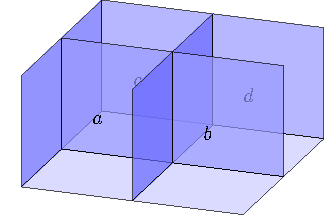
\includegraphics{1.pdf}
\end{center}

Lo mismo sucede con $B$, pero a esta se le agrega una nueva dimensión, sin cambiar el orden de sus elementos. Es decir, solo se pasa la representación bidimensional a una tridimensional tal que:

\begin{center}
    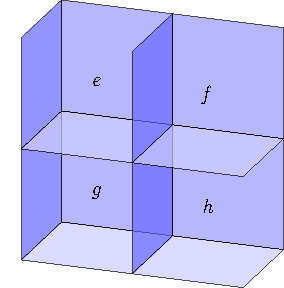
\includegraphics{2.pdf}
\end{center}

Después, esta forma se transpone internamente resultando en que $B_{ext}$ sea:

\begin{center}
    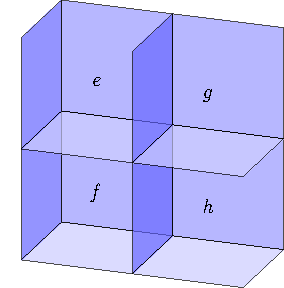
\includegraphics{3.pdf}
\end{center}

Ahora estas 2 formas se multiplican. La manera en al que sucede esto es elemento por elemento, dimensión por dimensión. Para una representación más visual, considere que la siguiente figura.

\begin{center}
    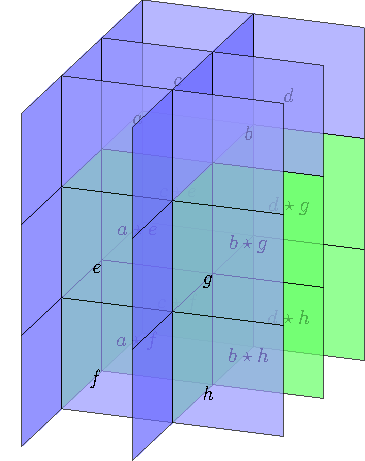
\includegraphics{4.pdf}
\end{center}

Como se puede ver, $A_{ext}$ toma su lugar en la parte superior y $B_{ext}$ se encuentra en la parte frontal. A partir de esto se puede considerar que cada variable es un factor de multiplicación en todas las celdas que tenga debajo o detrás de ella, dependiendo de su pertenencia en $A_{ext}$ o $B_{ext}$. Los cubos verdes indican los resultados de multiplicar estos factores pertenecientes a cada matriz. Enfocándose únicamente en los cubos verdes se obtiene el siguiente resultado:

\begin{center}
    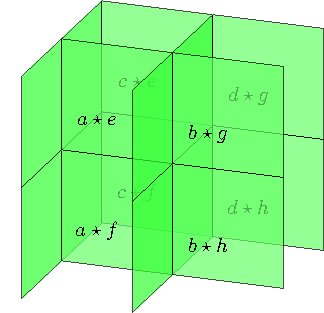
\includegraphics{5.pdf}
\end{center}

Esto significa que todas las multiplicaciones necesarias ya están presentes en la matriz y solo es necesario agregarlas la una a la otra para obtener el resultado deseado. Como se muestra en el código, está adición se lleva a cabo en el tercer eje (0, 1, 2), que corresponde a la dimensión horizontal (hacia la derecha o a la izquierda). Por lo tanto, el resultado es el siguiente:

\begin{center}
    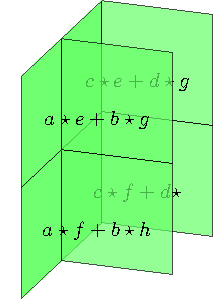
\includegraphics{6.pdf}
\end{center}

Debido a la manera en la que actúa \texttt{np.reduce}, una dimensión se elimina y la dimensión vertical tiene prioridad sobre la dimensión de profundidad, por lo tanto, se obtiene la matriz bidimensional vista al inicio:

$$
\begin{pmatrix}
    a \star e + b \star g & a \star f + b \star h \\
    c \star e + d \star g & c \star f + d \star h
\end{pmatrix}
$$

Este método tiene un mejor rendimiento que la suma iterativa de los elementos de renglones y columnas. No reduce el número de operaciones necesarias para computar la matriz resultante (como el algoritmo de \textit{Strassen} o el algoritmo de \textit{AlphaEvolve}), pero al utilizar diversas funciones internas de \textit{Numpy}, como la multiplicación normal (por \textit{*}) de 2 matrices y \texttt{np.reduce}, se logra un mejor rendimiento.

\section{Bibliografía}

\noindent\hangindent=2em \hangafter=1
Albert, V. V., \& Faist, P. (s.f.). \textit{Error Correction Zoo}. errorcorrectionzoo.org. https://errorcorrectionzoo.org/list/classical. \\

\noindent\hangindent=2em \hangafter=1
Axler, S. (2025). \textit{Linear Algebra Done Right - Fourth Edition}. Springer. https://linear.axler.net/LADR4e.pdf.\\

\noindent\hangindent=2em \hangafter=1
Hamming, R. W. (1950). Error Detecting and Error Correcting Codes. \textit{The Bell Systems Technical Journal, 20(2), 147-160}. https://zoo.cs.yale.edu/classes\\/cs323/doc/Hamming.pdf. \\

\noindent\hangindent=2em \hangafter=1
Sanderson, G. [3Blue1Brown]. (2020). \textit{But what are Hamming codes? The origin of error correction} [Vídeo]. YouTube. https://youtu.be/X8jsijhllIA?si=\\hh0OsmdzZ0MyK9ul. \\

\noindent\hangindent=2em \hangafter=1
Sanderson, G. [3Blue1Brown]. (2020). \textit{Hamming codes part 2: The one-line implementation} [Vídeo]. YouTube. https://youtu.be/b3NxrZOu\_CE?si=xuu\\KJ3WAlbdnc8cA. \\

\end{document}
